\chapter{Antecedentes y Estado del Arte}

En este capítulo se analizan los antecedentes y el estado del arte relacionados con el proyecto \textit{\textbf{NeuroForge}}. Para ello, se realiza un recorrido por la evolución de los juegos de estrategia desde sus orígenes en los juegos de mesa clásicos hasta sus adaptaciones modernas, tanto físicas como digitales. Este análisis permite identificar las mecánicas fundamentales que han influido en el diseño del proyecto, así como contextualizar las decisiones adoptadas durante su desarrollo.

\section{Evolución de los juegos de estrategia}

Desde la antigüedad, los juegos de mesa han servido como una representación lúdica del conflicto, la planificación y la toma de decisiones. En las primeras civilizaciones, estos juegos cumplían una función tanto recreativa como cultural, y sentaron las bases de conceptos estratégicos que perduran hasta la actualidad.

Entre los ejemplos más antiguos se encuentra el \textit{Juego Real de Ur}, originario de Iraq (aprox. del 2600-2400 a.C) \cite{BritishMuseumRoyalGameOfUr}, presentaba un tablero dividido en secciones conectadas, tal y como se muestra en la Figura~\ref{fig:JuegoRealDeUr}. Este diseño introducía decisiones tácticas relacionadas con el avance y la protección de las piezas, reforzando la importancia de la planificación a medio plazo. Ambos juegos, pese a su dependencia parcial del azar, contribuyeron a establecer una base conceptual sobre la que evolucionarían juegos de estrategia más complejos.

Aunque no se ha conservado un reglamento completo que permita reconstruir con total precisión las normas del juego, sí existe una descripción parcial recogida en una tablilla cuneiforme de origen babilonio, escrita entre los años 177 y 176 a.C. por el escriba Itti-Marduk-Balāṭu \cite{TheRoyalGameOfUrHistory}. A partir de este testimonio y de los tableros conservados, se considera que el Juego Real de Ur consistía en una competición entre dos jugadores en forma de carrera a lo largo del tablero, con mecánicas comparables a juegos actuales como el parchís o el backgammon.

De forma similar, el juego egipcio \textit{Senet}, documentado arqueológicamente durante el Imperio Nuevo, con ejemplares datados en el reinado de Amenhotep III (aprox. 1390--1353 a.C.) \cite{BrooklynMuseumSenet}, se desarrollaba sobre un tablero de treinta casillas, como se observa en la Figura~\ref{fig:Senet}. El desplazamiento de las piezas se determinaba mediante el lanzamiento de palos de conteo o huesos, introduciendo un componente de azar en la cantidad de casillas que podían avanzarse en cada turno. No obstante, el jugador conservaba un grado significativo de control estratégico, ya que podía decidir qué pieza mover, bloquear el avance del oponente o forzar retrocesos en determinadas situaciones. Esta combinación de aleatoriedad en la generación de movimientos y toma de decisiones tácticas en su aplicación convierte a \textit{Senet} en uno de los primeros ejemplos conocidos de juego que equilibra azar y planificación. Aunque su mecánica era relativamente simple, introducía ya la idea de progresión de piezas y competición directa entre jugadores, aspectos clave en el desarrollo temprano del pensamiento estratégico \cite{SenetHistory}.

Ambos juegos, pese a su dependencia parcial del azar, contribuyeron a establecer una base conceptual sobre la que evolucionarían juegos de estrategia más complejos.

Con el avance del tiempo, los juegos de estrategia comenzaron a abandonar progresivamente la dependencia del azar para centrarse en la planificación deliberada y la toma de decisiones informadas. En este contexto surge el \textit{Ajedrez}, cuyo origen se sitúa en la India alrededor del siglo VI d.C., a partir del juego conocido como \textit{Chaturanga} \cite{ChessHistory}. A diferencia de los juegos antiguos basados en carreras o desplazamientos condicionados por el azar, el ajedrez introduce una jerarquía claramente definida de piezas con capacidades diferenciadas y un sistema de captura directa. Estas características refuerzan conceptos como el sacrificio estratégico, el control del espacio y la planificación táctica a largo plazo. Asimismo, el ajedrez se caracteriza por ofrecer información completa a ambos jugadores, lo que lo convierte en un paradigma de la estrategia basada exclusivamente en la anticipación y el cálculo.

Dentro de esta evolución resulta especialmente relevante el juego chino \textit{Dou Shou Qi}, también conocido como \textit{Selva} o \textit{Ajedrez animal}. A diferencia de juegos clásicos cuya antigüedad está bien documentada, el origen histórico de \textit{Dou Shou Qi} no se encuentra claramente establecido. Las fuentes disponibles lo describen como un juego tradicional chino desarrollado con posterioridad al \textit{Xiangqi}, del que probablemente deriva a nivel conceptual \cite{ChessVariantsDouShouQi}.

El juego se estructura en torno a una jerarquía asimétrica de unidades representadas por animales, cada uno con un rango definido, y emplea un sistema de captura por desplazamiento similar al de los juegos de ajedrez (Tablero en la Figura~\ref{fig:DouShouQi}). No obstante, introduce excepciones explícitas en las reglas de captura —como la capacidad de una pieza de rango inferior para derrotar a otra superior bajo determinadas condiciones—, lo que rompe la jerarquía estricta y añade una dimensión estratégica basada en la gestión del riesgo y la anticipación del comportamiento del oponente. Este tipo de jerarquía no lineal anticipa principios fundamentales que aparecerán más adelante en los juegos de estrategia militar modernos.

El siguiente paso se produce a comienzos del siglo XX con la aparición de \textit{L’Attaque}, un juego de mesa diseñado por Hermance Edan, quien registró su patente el 26 de noviembre de 1908 \cite{BAdaLAttaque}. En su descripción original, el juego se define como un \textit{«jeu de bataille avec des pièces mobiles sur damier»}, es decir, un juego de batalla con piezas móviles sobre un tablero cuadriculado (Figura~\ref{fig:lattaque}). La patente fue publicada oficialmente en 1909 por la Oficina de Patentes francesa, y el juego fue comercializado de forma continuada desde ese año hasta comienzos de la década de 1930.

\textit{L’Attaque} introduce por primera vez de manera explícita la ocultación de información como mecánica central del diseño. Cada jugador dispone de un conjunto de piezas con valores numéricos jerárquicos, cuyo rango permanece oculto al oponente hasta el momento de la confrontación directa. El resultado del combate se resuelve comparando los valores de las piezas implicadas, eliminándose generalmente la de menor rango. La partida concluye cuando uno de los jugadores localiza y captura la pieza objetivo del adversario, identificada como la bandera.

Estas mecánicas suponen una ruptura clara con los juegos de información completa predominantes hasta ese momento, al trasladar una parte sustancial de la toma de decisiones al ámbito de la inferencia, el engaño y la gestión del riesgo. Asimismo, \textit{L’Attaque} consolida una jerarquía militar explícita y permite la configuración libre de la disposición inicial de las unidades, lo que incrementa la profundidad estratégica desde el primer turno y refuerza la importancia de la planificación previa. En conjunto, estas innovaciones marcan un punto de inflexión en el diseño de juegos de estrategia, al introducir por primera vez de forma sistemática la incertidumbre como recurso estratégico.

La progresión histórica desde los primeros juegos de mesa hasta títulos como \textit{L’Attaque} pone de manifiesto una evolución gradual desde mecánicas dominadas por el azar y el movimiento lineal hacia sistemas estratégicos cada vez más complejos, basados en la jerarquía de unidades, la confrontación directa y, finalmente, la ocultación de información. Esta acumulación progresiva de conceptos estratégicos, planificación, gestión del riesgo, engaño e inferencia, configura el marco teórico sobre el que se desarrollaría posteriormente \textit{Stratego} y, por extensión, fundamenta las decisiones de diseño del proyecto \textit{\textbf{NeuroForge}}.

% Revisado hasta aqui

\section{El juego original: \textit{Stratego}}

El juego \textit{Stratego} constituye uno de los referentes más influyentes dentro del ámbito de los juegos de estrategia con información imperfecta. Su diseño no surge de forma aislada, sino que se apoya en una serie de innovaciones mecánicas desarrolladas a comienzos del siglo XX, especialmente a partir del juego europeo \textit{L’Attaque}, considerado su antecedente directo.

La versión moderna de \textit{Stratego} fue desarrollada tras la Segunda Guerra Mundial por la compañía neerlandesa Jumbo, que adoptó una estética de inspiración militar napoleónica. El juego fue registrado comercialmente en 1960 y su difusión internacional se consolidó en 1961, cuando Milton Bradley obtuvo la licencia para su distribución en Estados Unidos \cite{StrategoHistoryUltraBoardGames}.

Desde el punto de vista mecánico, \textit{Stratego} se articula en torno a una jerarquía militar explícita de unidades, cuyos rangos permanecen ocultos al oponente hasta el momento del enfrentamiento directo. El sistema de combate se resuelve mediante la comparación de los valores de las piezas implicadas, eliminándose generalmente la de menor rango. El objetivo principal de la partida consiste en localizar y capturar la pieza objetivo del adversario, identificada como la bandera.

Una de las decisiones de diseño más relevantes es la configuración inicial libre del despliegue de las unidades, que traslada una parte sustancial del peso estratégico al momento previo al inicio de la partida. Esta característica, combinada con la ocultación de información, fomenta el engaño, la deducción y la gestión del riesgo como elementos centrales de la experiencia de juego.

Desde el punto de vista material, \textit{Stratego} ha experimentado diversas adaptaciones físicas a lo largo del tiempo. Las primeras ediciones utilizaban piezas de cartón impreso, que fueron sustituidas posteriormente por piezas de madera pintada. A partir de finales de la década de 1960, estas fueron reemplazadas por piezas de plástico, más económicas y estables. Este cambio no solo respondió a criterios de producción, sino que también redujo el riesgo de vuelco accidental de las piezas, un problema crítico en un juego donde la revelación involuntaria de la información compromete el desarrollo estratégico de la partida.

Desde una perspectiva de diseño, \textit{Stratego} se caracteriza por la ausencia total de elementos aleatorios durante la partida. Todas las decisiones se basan en la planificación, la inferencia y la lectura del comportamiento del oponente, lo que lo convierte en un paradigma de la estrategia bajo información imperfecta. Estas características explican su influencia duradera y justifican su elección como principal referencia conceptual y base del diseño para el desarrollo del proyecto \textit{\textbf{NeuroForge}}.

\section{Variaciones, adaptaciones y videojuegos relacionados}

Además de sus múltiples ediciones físicas, \textit{Stratego} ha dado lugar a numerosas variantes temáticas ambientadas en universos de ficción como \textit{Star Wars}, \textit{El Señor de los Anillos}, o \textit{Marvel}. Estas adaptaciones mantienen la estructura básica del juego original, introduciendo cambios estéticos y ajustes menores en las reglas según la ambientación.

En el ámbito digital, \textit{Stratego} cuenta con versiones en línea que permiten partidas a distancia entre jugadores de todo el mundo como el \textit{Stratego Online}\footnote{\url{ https://www.stratego.com}} y apps móviles disponibles en iOS y Android. Estas plataformas incorporan modos clásicos y variantes con tableros alternativos o un número reducido de piezas, contribuyendo a mantener vigente el interés por el juego. El juego conserva además presencia activa en el ámbito competitivo, especialmente en países como Países Bajos, Alemania y Bélgica, Incluyendo torneos oficiales y rankings europeos.

Junto a \textit{Stratego}, existen otros juegos de mesa y digitales basados en principios similares. Un ejemplo es \textit{Luzhanqi} \cite{LuzhanqiHistory}, originario de China, cuyo tablero se muestra en la Figura~\ref{fig:Luzhanqi}. Este juego comparte la mecánica de piezas ocultas y configuración libre inicial, evidenciando una convergencia de ideas estratégicas entre distintas tradiciones culturales.

En el ámbito de los videojuegos, destacan títulos de estrategia por turnos que enfatizan la planificación, la jerarquía de unidades y la toma de decisiones en entornos discretos. Entre ellos se encuentran la saga \textit{Advance Wars} (Intelligent Systems, Advance Wars series, Nintendo) y \textit{Into the Breach} (Subset Games, Into the Breach). En ambos casos, aunque la información sobre el enemigo es visible, el peso estratégico recae en la gestión de unidades, el posicionamiento y la anticipación de las acciones del rival.

Dentro del ámbito de los videojuegos de estrategia por turnos que comparten principios mecánicos con \textit{Stratego}, destacan títulos como la saga \textit{Advance Wars}. Esta serie, desarrollada por Intelligent Systems para plataformas de Nintendo entre 2001 y 2019, se basa en combates tácticos sobre un tablero cuadriculado donde los jugadores despliegan y gestionan unidades con jerarquías y características diferenciadas. Cada unidad posee fortalezas y debilidades específicas frente a otros tipos de unidades, lo que obliga a planificar los movimientos cuidadosamente y anticipar las acciones del adversario. Aunque la información sobre la ubicación de las unidades enemigas es visible, la profundidad estratégica recae en la gestión eficiente de recursos, el posicionamiento táctico y la secuencia de ataques, elementos que recuerdan la planificación y la jerarquía presentes en \textit{Stratego}.

De manera similar, el videojuego \textit{Into the Breach} (Subset Games, 2018) traslada el concepto de estrategia por turnos a un entorno de tablero discretizado donde cada unidad tiene capacidades específicas y limitadas. La mecánica principal consiste en anticipar el comportamiento del enemigo y planificar acciones para proteger objetivos clave, equilibrando riesgo y recompensa en cada turno. Esta combinación de toma de decisiones estrictamente calculada, jerarquía de unidades y confrontación directa recuerda la esencia de \textit{Stratego}, donde el control del espacio y la gestión de las piezas son determinantes para la victoria. La simplicidad aparente del tablero contrasta con la profundidad estratégica requerida, consolidando a \textit{Into the Breach} como un ejemplo contemporáneo de cómo los principios clásicos de los juegos de estrategia pueden adaptarse eficazmente al medio digital.

Estas aproximaciones digitales ponen de manifiesto la diversidad de soluciones adoptadas en el diseño de videojuegos de estrategia y sirven como referencia para el desarrollo de \textit{\textbf{NeuroForge}}. El objetivo del proyecto es combinar la jerarquía de unidades y la confrontación directa propias de \textit{Stratego} con las ventajas del medio digital, manteniendo la tensión estratégica derivada de la información oculta y aprovechando las posibilidades de automatización, accesibilidad y escalabilidad que ofrece el formato de videojuego.

\section{Motor de videojuegos utilizado}

Los motores de videojuegos funcionan como un \textit{framework} de desarrollo, proporcionando un conjunto integrado de herramientas, librerías y sistemas que sirven como base tecnológica para la creación de un videojuego. Estos motores abstraen gran parte de la complejidad técnica inherente al desarrollo, ofreciendo soluciones ya implementadas para tareas como el renderizado gráfico, la gestión de escenas, el control de entrada del usuario, la simulación de físicas o la exportación a distintas plataformas. Gracias a esta abstracción, el desarrollador puede centrarse principalmente en la lógica del juego, el diseño de mecánicas y la experiencia del usuario.

La elección del motor de videojuegos influye de manera directa en el proceso de desarrollo y en las características finales del producto. Factores como el flujo de trabajo, el rendimiento, la escalabilidad, la facilidad de mantenimiento del código y los tiempos de implementación están fuertemente condicionados por las herramientas y la arquitectura que ofrece el motor seleccionado. En el contexto de un proyecto académico individual, esta decisión cobra especial relevancia, ya que deben considerarse además aspectos como la curva de aprendizaje, la disponibilidad de documentación y recursos, y la adecuación del motor al alcance real del proyecto.

Con el objetivo de seleccionar el motor más adecuado para el desarrollo del videojuego \textit{NeuroForge}, se realizó un análisis comparativo inicial de tres de los motores de desarrollo más utilizados en la actualidad: Unreal Engine, Unity y Godot. Estos motores cuentan con una amplia presencia tanto en el ámbito profesional como en el educativo y representan diferentes enfoques dentro del desarrollo de videojuegos \cite{rocketbrush_engines_2025}.

Para realizar esta comparación se han considerado varios criterios relevantes para el contexto del proyecto. Entre ellos destacan el rendimiento del motor, la facilidad de aprendizaje, la adecuación al desarrollo de videojuegos en dos dimensiones, los requisitos de hardware, el ecosistema de herramientas disponibles y el modelo de licencias.

Unreal Engine es uno de los motores más utilizados dentro de la industria del videojuego, especialmente en producciones de gran presupuesto y alta exigencia gráfica. Sus avanzados sistemas de renderizado, iluminación y simulación física permiten desarrollar entornos tridimensionales altamente realistas, lo que lo convierte en una herramienta especialmente adecuada para proyectos de gran escala y alta fidelidad visual. Sin embargo, esta potencia técnica implica también una mayor complejidad en el flujo de trabajo y una curva de aprendizaje más pronunciada, especialmente para desarrolladores sin experiencia previa. Asimismo, los requerimientos de hardware suelen ser más elevados y los tiempos de compilación pueden resultar más largos en comparación con otros motores. Estas características pueden suponer una desventaja en proyectos académicos o desarrollos individuales donde el tiempo y los recursos disponibles son limitados.

Unity, por su parte, se ha consolidado como uno de los motores de videojuegos más populares tanto en el ámbito independiente como en el educativo. Su principal ventaja radica en su versatilidad, ya que permite desarrollar videojuegos en dos y tres dimensiones para una amplia variedad de plataformas. Además, cuenta con una comunidad muy extensa, una gran cantidad de documentación disponible y un ecosistema amplio de herramientas, extensiones y recursos que facilitan el aprendizaje y aceleran el desarrollo. No obstante, algunos análisis técnicos señalan que en proyectos con estructuras complejas o con altas exigencias gráficas pueden aparecer problemas de rendimiento si no se realiza una gestión cuidadosa de los recursos. Asimismo, aunque Unity ofrece soporte para el desarrollo bidimensional, su arquitectura interna está históricamente orientada al desarrollo tridimensional, lo que puede introducir cierta sobrecarga innecesaria en proyectos 2D más sencillos.

Finalmente, Godot es un motor de desarrollo de código abierto que ha ganado una notable popularidad en los últimos años, especialmente dentro del desarrollo independiente y el ámbito educativo. Su filosofía se basa en la simplicidad, la modularidad y la accesibilidad, lo que facilita su uso en proyectos de pequeña y mediana escala. Una de sus principales características es su arquitectura basada en nodos, que favorece un diseño modular y fácilmente mantenible del sistema. Además, Godot ofrece herramientas especialmente sólidas para el desarrollo de videojuegos en dos dimensiones, permitiendo ciclos de desarrollo rápidos y un prototipado ágil. A esto se suma la ausencia de costes de licencia y el acceso completo a su código fuente, lo que permite una mayor libertad de experimentación. Como principal limitación, el motor presenta capacidades menos maduras en el desarrollo de entornos tridimensionales complejos en comparación con motores comerciales como Unreal Engine o Unity, así como un ecosistema de extensiones más reducido.

La Tabla \ref{tab:comparativa_motores} resume de forma sintética las principales características de los motores analizados, considerando los criterios más relevantes para el desarrollo del proyecto.

\begin{table}[H]
	\centering
	\begin{tabular}{|l|c|c|c|}
		\hline
		\textbf{Criterio} & \textbf{Unreal Engine} & \textbf{Unity} & \textbf{Godot} \\
		\hline
		Rendimiento en 3D & Muy alto & Alto & Medio \\
		\hline
		Rendimiento en 2D & Medio & Alto & Muy alto \\
		\hline
		Curva de aprendizaje & Alta & Media & Baja \\
		\hline
		Requisitos de hardware & Altos & Medios & Bajos \\
		\hline
		Modelo de licencia & Comercial & Comercial & Código abierto \\
		\hline
		Adecuación a proyectos individuales & Media & Alta & Muy alta \\
		\hline
		Ecosistema y comunidad & Muy amplio & Muy amplio & En crecimiento \\
		\hline
	\end{tabular}
	\caption{Comparativa entre motores de desarrollo de videojuegos}
	\label{tab:comparativa_motores}
\end{table}

Tras el análisis realizado, se ha determinado que Godot es el motor más adecuado para el desarrollo del proyecto \textit{NeuroForge}. Dado que se trata de un videojuego de estrategia por turnos en dos dimensiones, con un alcance controlado y desarrollado en un contexto académico individual, las ventajas de Godot en términos de simplicidad, rendimiento en 2D y ausencia de costes de licencia superan claramente sus limitaciones técnicas.

Además, su ligereza y rapidez en los ciclos de desarrollo favorecen un enfoque iterativo basado en pruebas frecuentes y refinamiento progresivo, lo que resulta especialmente adecuado para un proyecto desarrollado por una única persona y alineado con la metodología de trabajo adoptada en este TFG.

\begin{figure}[h!]
	\centering
	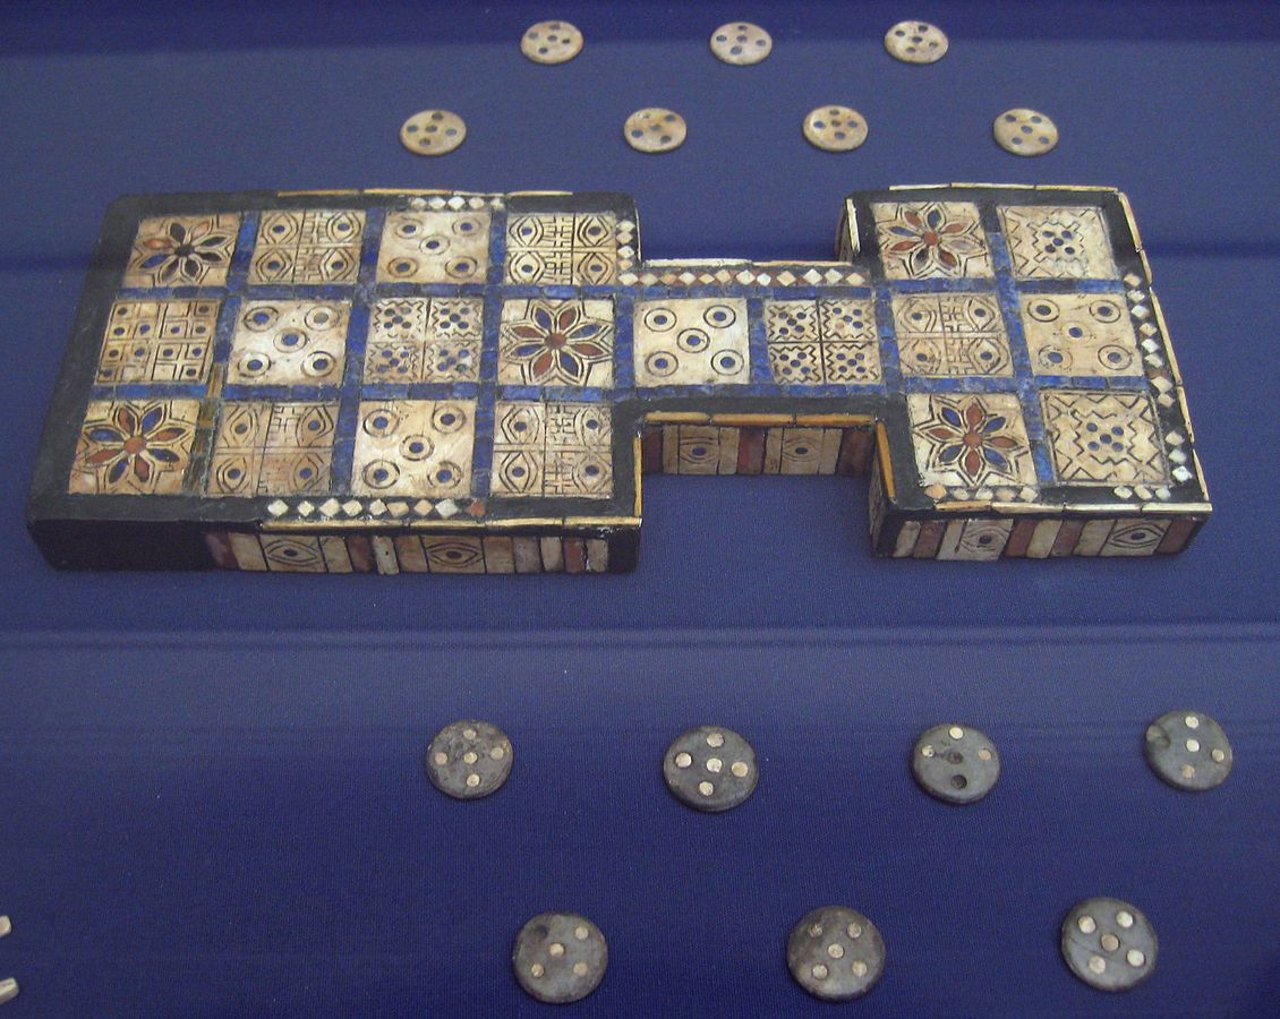
\includegraphics[width=0.86\linewidth]{../Imagenes/JuegoRealDeUr.png}
	\caption{Tablero del Juego Real de Ur \cite{TheRoyalGameOfUrHistory}}
	\label{fig:JuegoRealDeUr}
\end{figure}

\begin{figure}[h!]
	\centering
	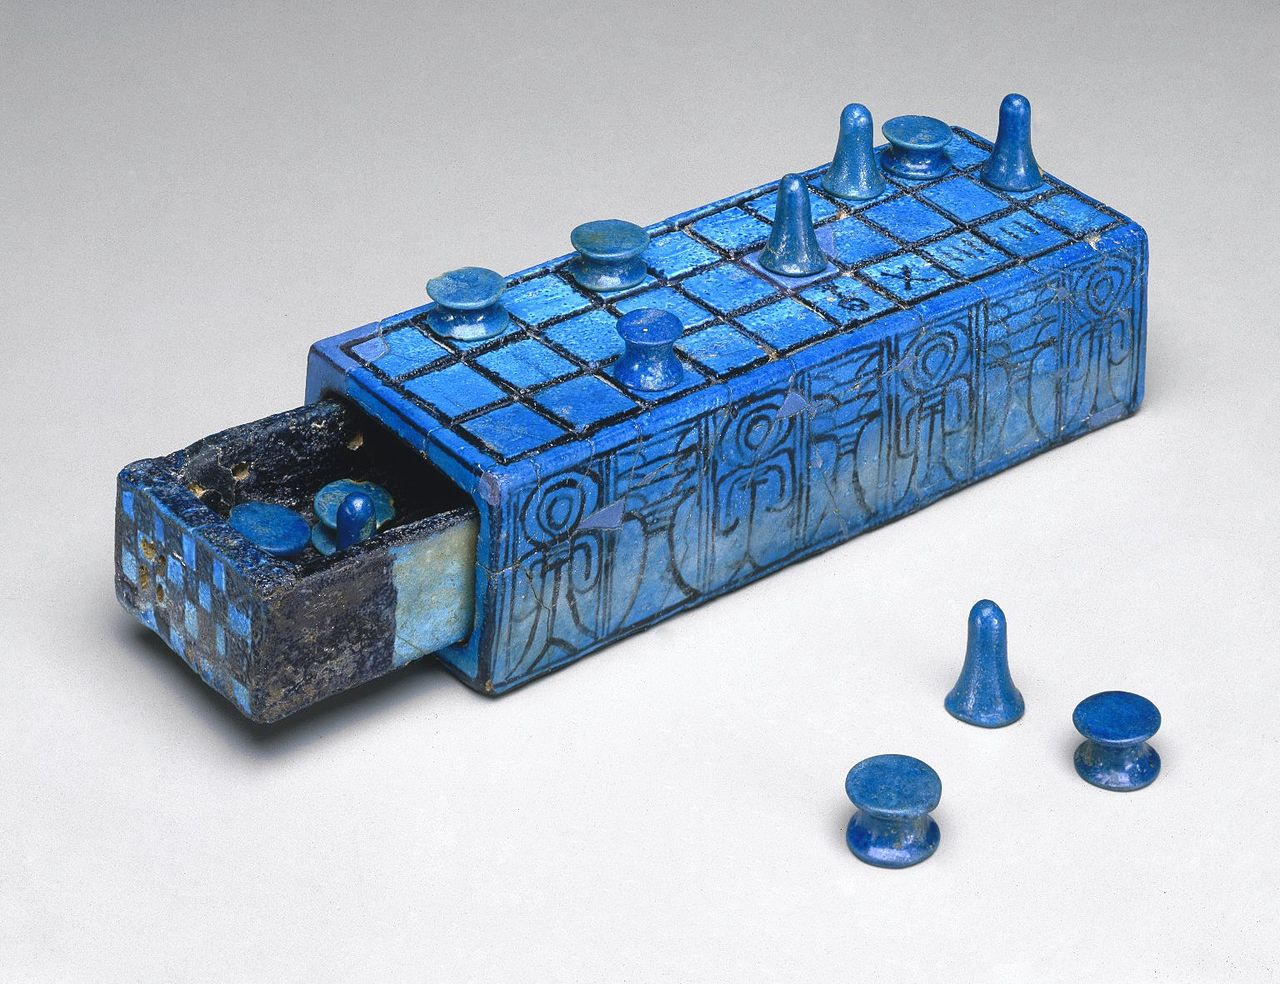
\includegraphics[width=0.86\linewidth]{../Imagenes/Senet.png}
	\caption{Tablero del juego Senet \cite{BrooklynMuseumSenet}}
	\label{fig:Senet}
\end{figure}

\begin{figure}[h!]
	\centering
	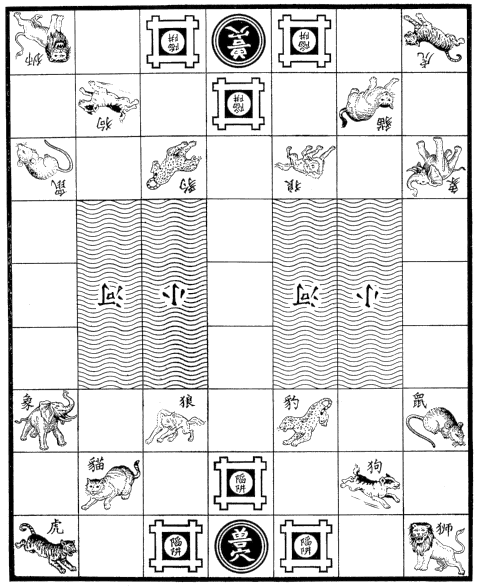
\includegraphics[width=0.86\linewidth]{../Imagenes/DouShouQi.png}
	\caption{Tablero del juego Dou Shou Qi \cite{ChessVariantsDouShouQi}}
	\label{fig:DouShouQi}
\end{figure}

\begin{figure}[h!]
	\centering
	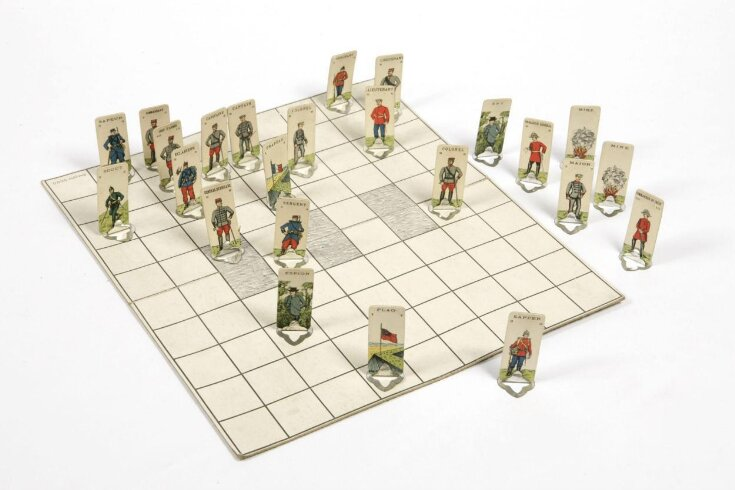
\includegraphics[width=0.86\linewidth]{../Imagenes/lattaque.png}
	\caption{Tablero del juego L'attaque \cite{LAttaqueBoard}}
	\label{fig:lattaque}
\end{figure}

\begin{figure}[h!]
	\centering
	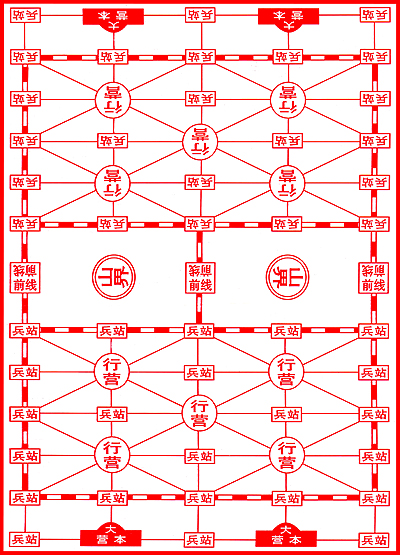
\includegraphics[width=0.86\linewidth]{../Imagenes/Luzhanqi.png}
	\caption{Tablero del juego Luzhanqi \cite{LuzhanqiHistory}}
	\label{fig:Luzhanqi}
\end{figure}



